\chapter{Wyniki oraz omówienie}
\label{chap:wyniki}

W celu porównania obu rozwiązań przedstawionych w \autoref{chap:implementacja} przeprowadzono szereg testów.
Oceniono poprawność działania algorytmu na uproszczonych, automatycznie generowanych danych a także na podstawie
rzeczywistych danych pochodzących ze skanowania laserowego. Sprawdzono również czasy przetwarzania dla poszczególnych
algorytmów oraz stwierdzono, czy możliwe jest wykorzystanie obu algorytmów jednocześnie w celu poprawienia jakości wyników.

Wszystkie testy zostały przeprowadzone na komputerze, którego specyfikacje podano w tabeli \ref{tab:specyfikacja}.

\begin{table}[h!]
    \centering
    \begin{tabular}{|p{0.5\linewidth}|p{0.5\linewidth}|}
        \hline
        Procesor & Intel Core i5-6300U 2,4 GHz \\
        \hline
		Pamieć & 16GB \\
		\hline
		Dysk & Intel SSDSC2BB80 800GB \\
		\hline
		System Operacyjny & Fedora 23 kernel 4.6.3 \\
		\hline
		Interpreter Pythona & Python 2.7.11 \\
		\hline
    \end{tabular}
    \caption{Specyfikacja platformy testowej}
    \label{tab:specyfikacja}
\end{table}

\section{Testy na danych wygenerowanych}
Pierwszy z testów miał wykazać poprawność działania zaimplementowanych algorytmów. W tym celu wygenerowano zbiór 1000 punktów,
których współrzędne $x,y \in <0,1>$, zaś wartość wspólrzędnej $z$ dana jest wzorem:

\begin{displaymath}
    z = \left\{ \begin{array}{ll}
        r & \textrm{$x < 0,4 \vee x > 0,6 \vee y < 0,4 \vee y > 0,6$}\\
        1 + r & \textrm{$0,4 < x < 0,6 \wedge 0,4 < y < 0,6$}\\
    \end{array} \right.
\end{displaymath}


Gdzie $r$ jest zmienna losową z przedziału $<0;0,1>$. Tak utworzone dane powinny zostać zintepretowane jako
dwie niezależne płaszczyzny. Widok przykładowych danych w 3 wymiarach pokazano na rysunku \ref{fig:dane_zerowe}.

\begin{figure}[h!]
    \centering
    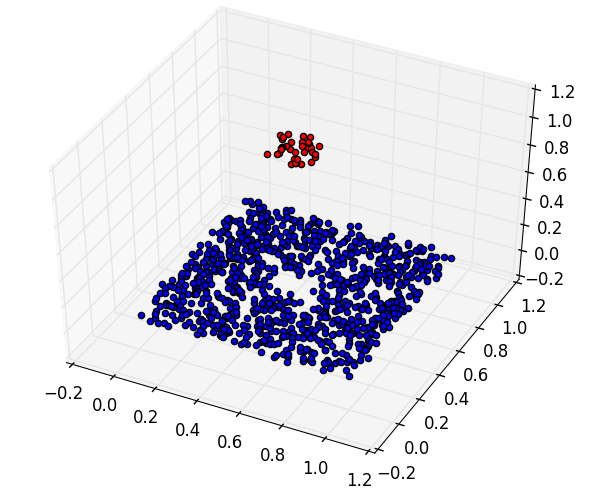
\includegraphics[width=0.6\linewidth]{img/test0.png}
    \caption{Dane testowe w rzucie 3D}
    \label{fig:dane_zerowe}
\end{figure}

Dane testowe oraz wyniki działania algorytmu przedstawiono na rysunkach \ref{fig:test1} i \ref{fig:test2}.
Przez kolor czerwony zostały oznaczone punkty dla których $z > 1$.

\begin{figure}[h!]
    \centering
    \begin{subfigure}[b]{0.5\linewidth}
        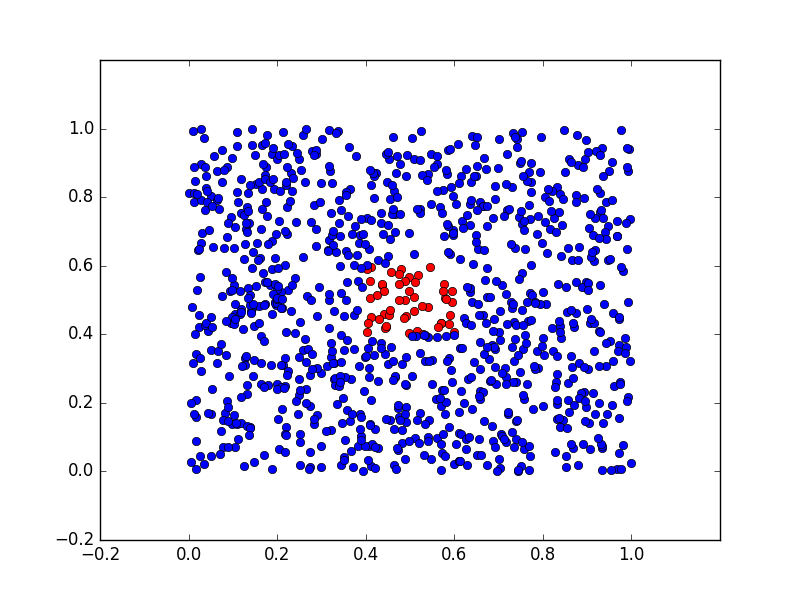
\includegraphics[width=\linewidth]{img/test1_1.png}
		\caption{Dane wejściowe}
    \end{subfigure}%
    \begin{subfigure}[b]{0.5\linewidth}
        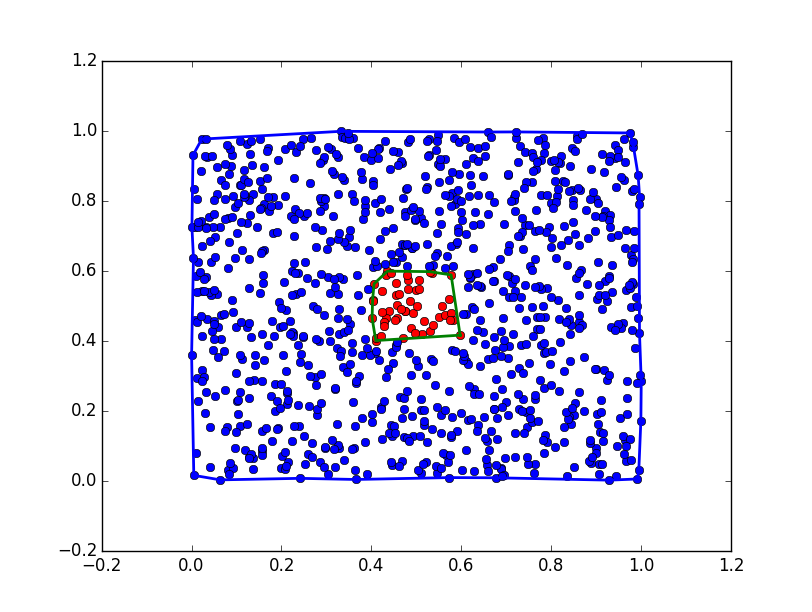
\includegraphics[width=\linewidth]{img/test1_2.png}
		\caption{Algorytm naiwny}
    \end{subfigure}%

    \begin{subfigure}[b]{0.5\linewidth}
        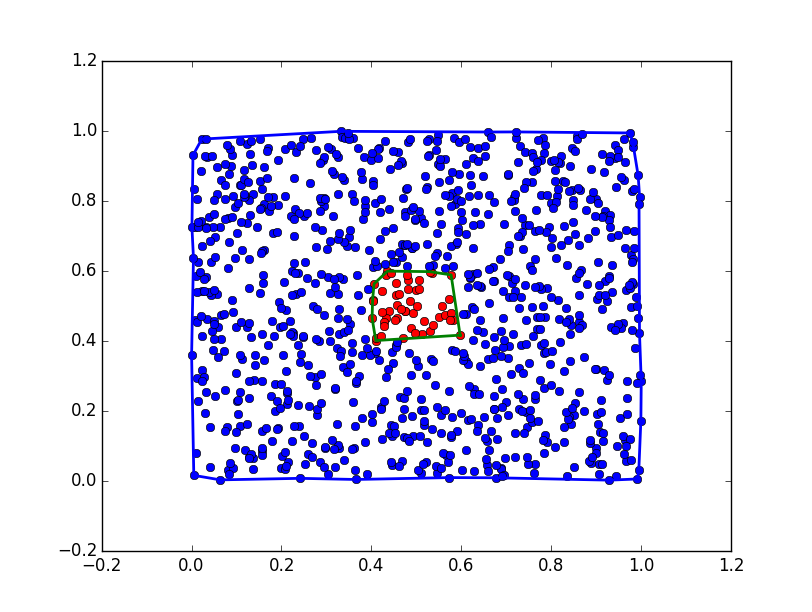
\includegraphics[width=\linewidth]{img/test1_3.png}
        \caption{Algorytm iteracyjny (1 iteracja)}
    \end{subfigure}%
    \caption{Wyniki działa algorytmu dla wygenerowanych danych testowych}
    \label{fig:test1}
\end{figure}

Jak widać na rysunku \ref{fig:test1} oba algorytmy poprawnie wykryły dwie powierzchnie. Co ciekawe,
algorytm iteracyjny już po pierwszej iteracji poprawnie zakwalifikował punkty do dwóch zbiorów. Niestety, jest to
dziełem przypadku, co pokazano na rysunku \ref{fig:test2}

\begin{figure}[h!]
    \centering
    \begin{subfigure}[b]{0.5\linewidth}
        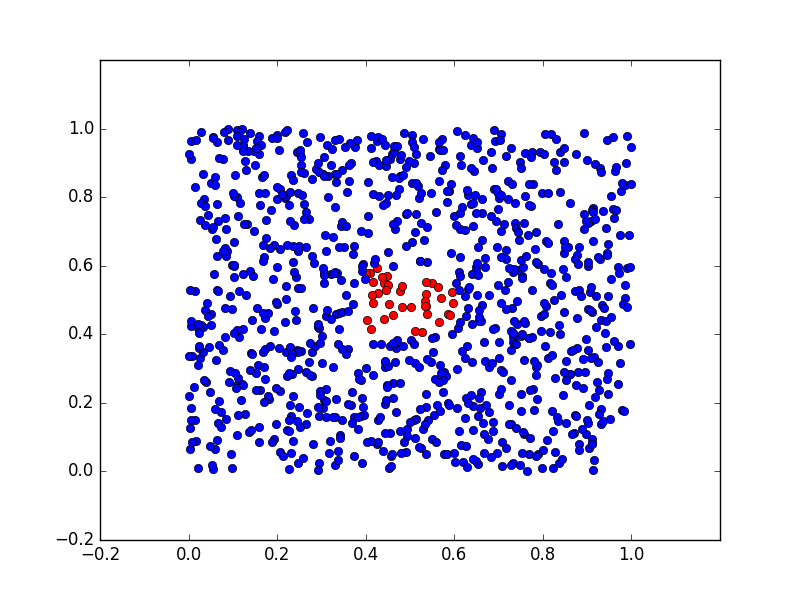
\includegraphics[width=\linewidth]{img/test2_1.png}
        \caption{Dane wejściowe}
    \end{subfigure}%
    \begin{subfigure}[b]{0.5\linewidth}
        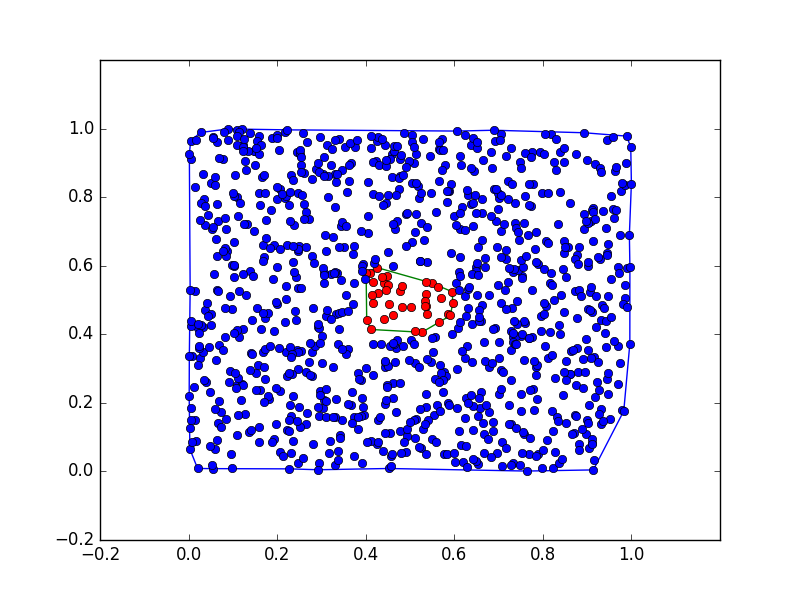
\includegraphics[width=\linewidth]{img/test2_2.png}
        \caption{Algorytm naiwny}
    \end{subfigure}%

    \begin{subfigure}[b]{0.5\linewidth}
        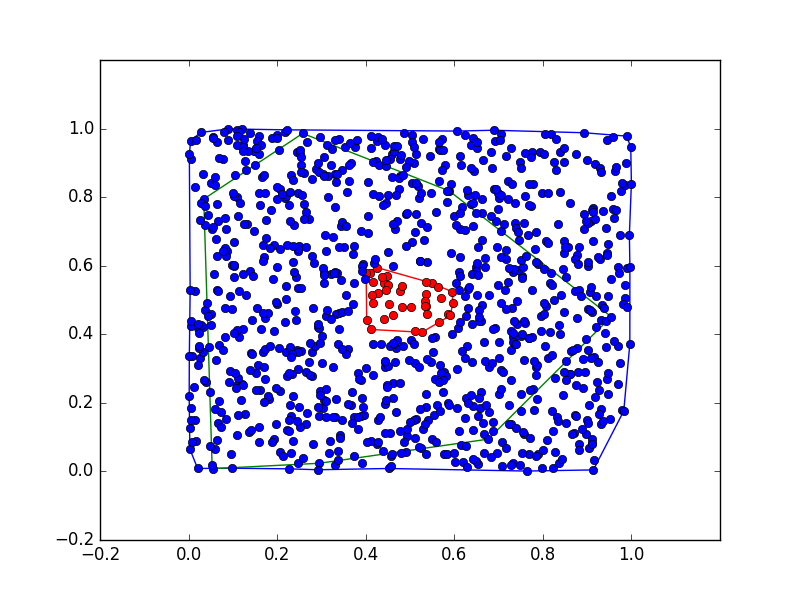
\includegraphics[width=\linewidth]{img/test2_3.png}
        \caption{Algorytm iteracyjny (1 iteracja)}
    \end{subfigure}%
    \begin{subfigure}[b]{0.5\linewidth}
        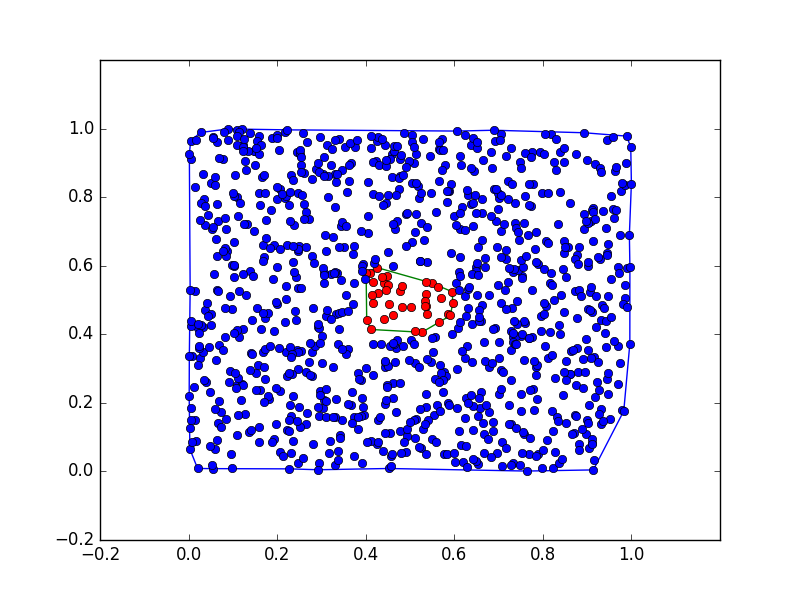
\includegraphics[width=\linewidth]{img/test2_4.png}
        \caption{Algorytm iteracyjny (7 iteracja)}
    \end{subfigure}%
    \caption{Wyniki działa algorytmu dla wygenerowanych danych testowych}
    \label{fig:test2}
\end{figure}

W przypadku pokazanym na rysunku \ref{fig:test2} koniecznych było 7 iteracji, aby w prawidłowy sposób wykryć, iż
w danych testowych znajdują się dwie powierzchnię. Przypadek ten pokazuje, że algorytm iteracyjny ma właściwości
poprawiania wyników wraz z kolejnymi iteracjami. Porównano także czasy wykonywania się algorytmów (tabela \ref{tab:czasy1})

\begin{table}[h!]
    \centering
    \begin{tabular}{|p{0.5\linewidth}|p{0.5\linewidth}|}
        \hline
        Algorytm Naiwny &  \\
        \hline
        Algorytm Iteracyjny (1 iteracja) & \\
        \hline
        Algorytm Iteracyjny (7 iteracji) & \\
        \hline
    \end{tabular}
    \caption{Średnie czasy wykonywania sie algorytmu}
    \label{tab:czasy1}
\end{table}



